%!TEX root=./LIVRO.tex
\setcounter{chapter}{0}
\chapter[Simulado 1]{Simulado}
\markboth{Simulado 1}{}

\vspace*{-1cm}

\num{1} VEJA O ANIMAL QUE BIA ENCONTROU NA PRAIA.

\begin{figure}[H]
\centering

\includegraphics[width=.5\textwidth]{./media/image210.jpg}
\end{figure}

A PALAVRA QUE SE INICIA COM A MESMA LETRA INICIAL É A MESMA DO NOME DESSE ANIMAL É

\begin{multicols}{2}
\begin{escolha}
\item VACA.

\item FADA.

\item TOCA.

\item DOCE.
\end{escolha}
\end{multicols}

\num{2} OBSERVE O UTENSÍLIO QUE PAULA GANHOU PARA SUA COZINHA.
\enlargethispage{2\baselineskip}

\begin{figure}[H]
\centering
\includegraphics[width=.5\textwidth]{./media/image211.jpg}
\end{figure}

A PALAVRA QUE SE INICIA COM A MESMA SÍLABA DO UTENSÍLIO É

\begin{multicols}{2}
\begin{escolha}
\item PAPAGAIO.

\item BANANA.

\item JANELA.

\item PETECA.
\end{escolha}
\end{multicols}

\pagebreak
\num{3} VEJA O MÓVEL QUE DONA LILI COMPROU NA LOJA DO SEU BAIRRO.

\begin{figure}[H]
\centering
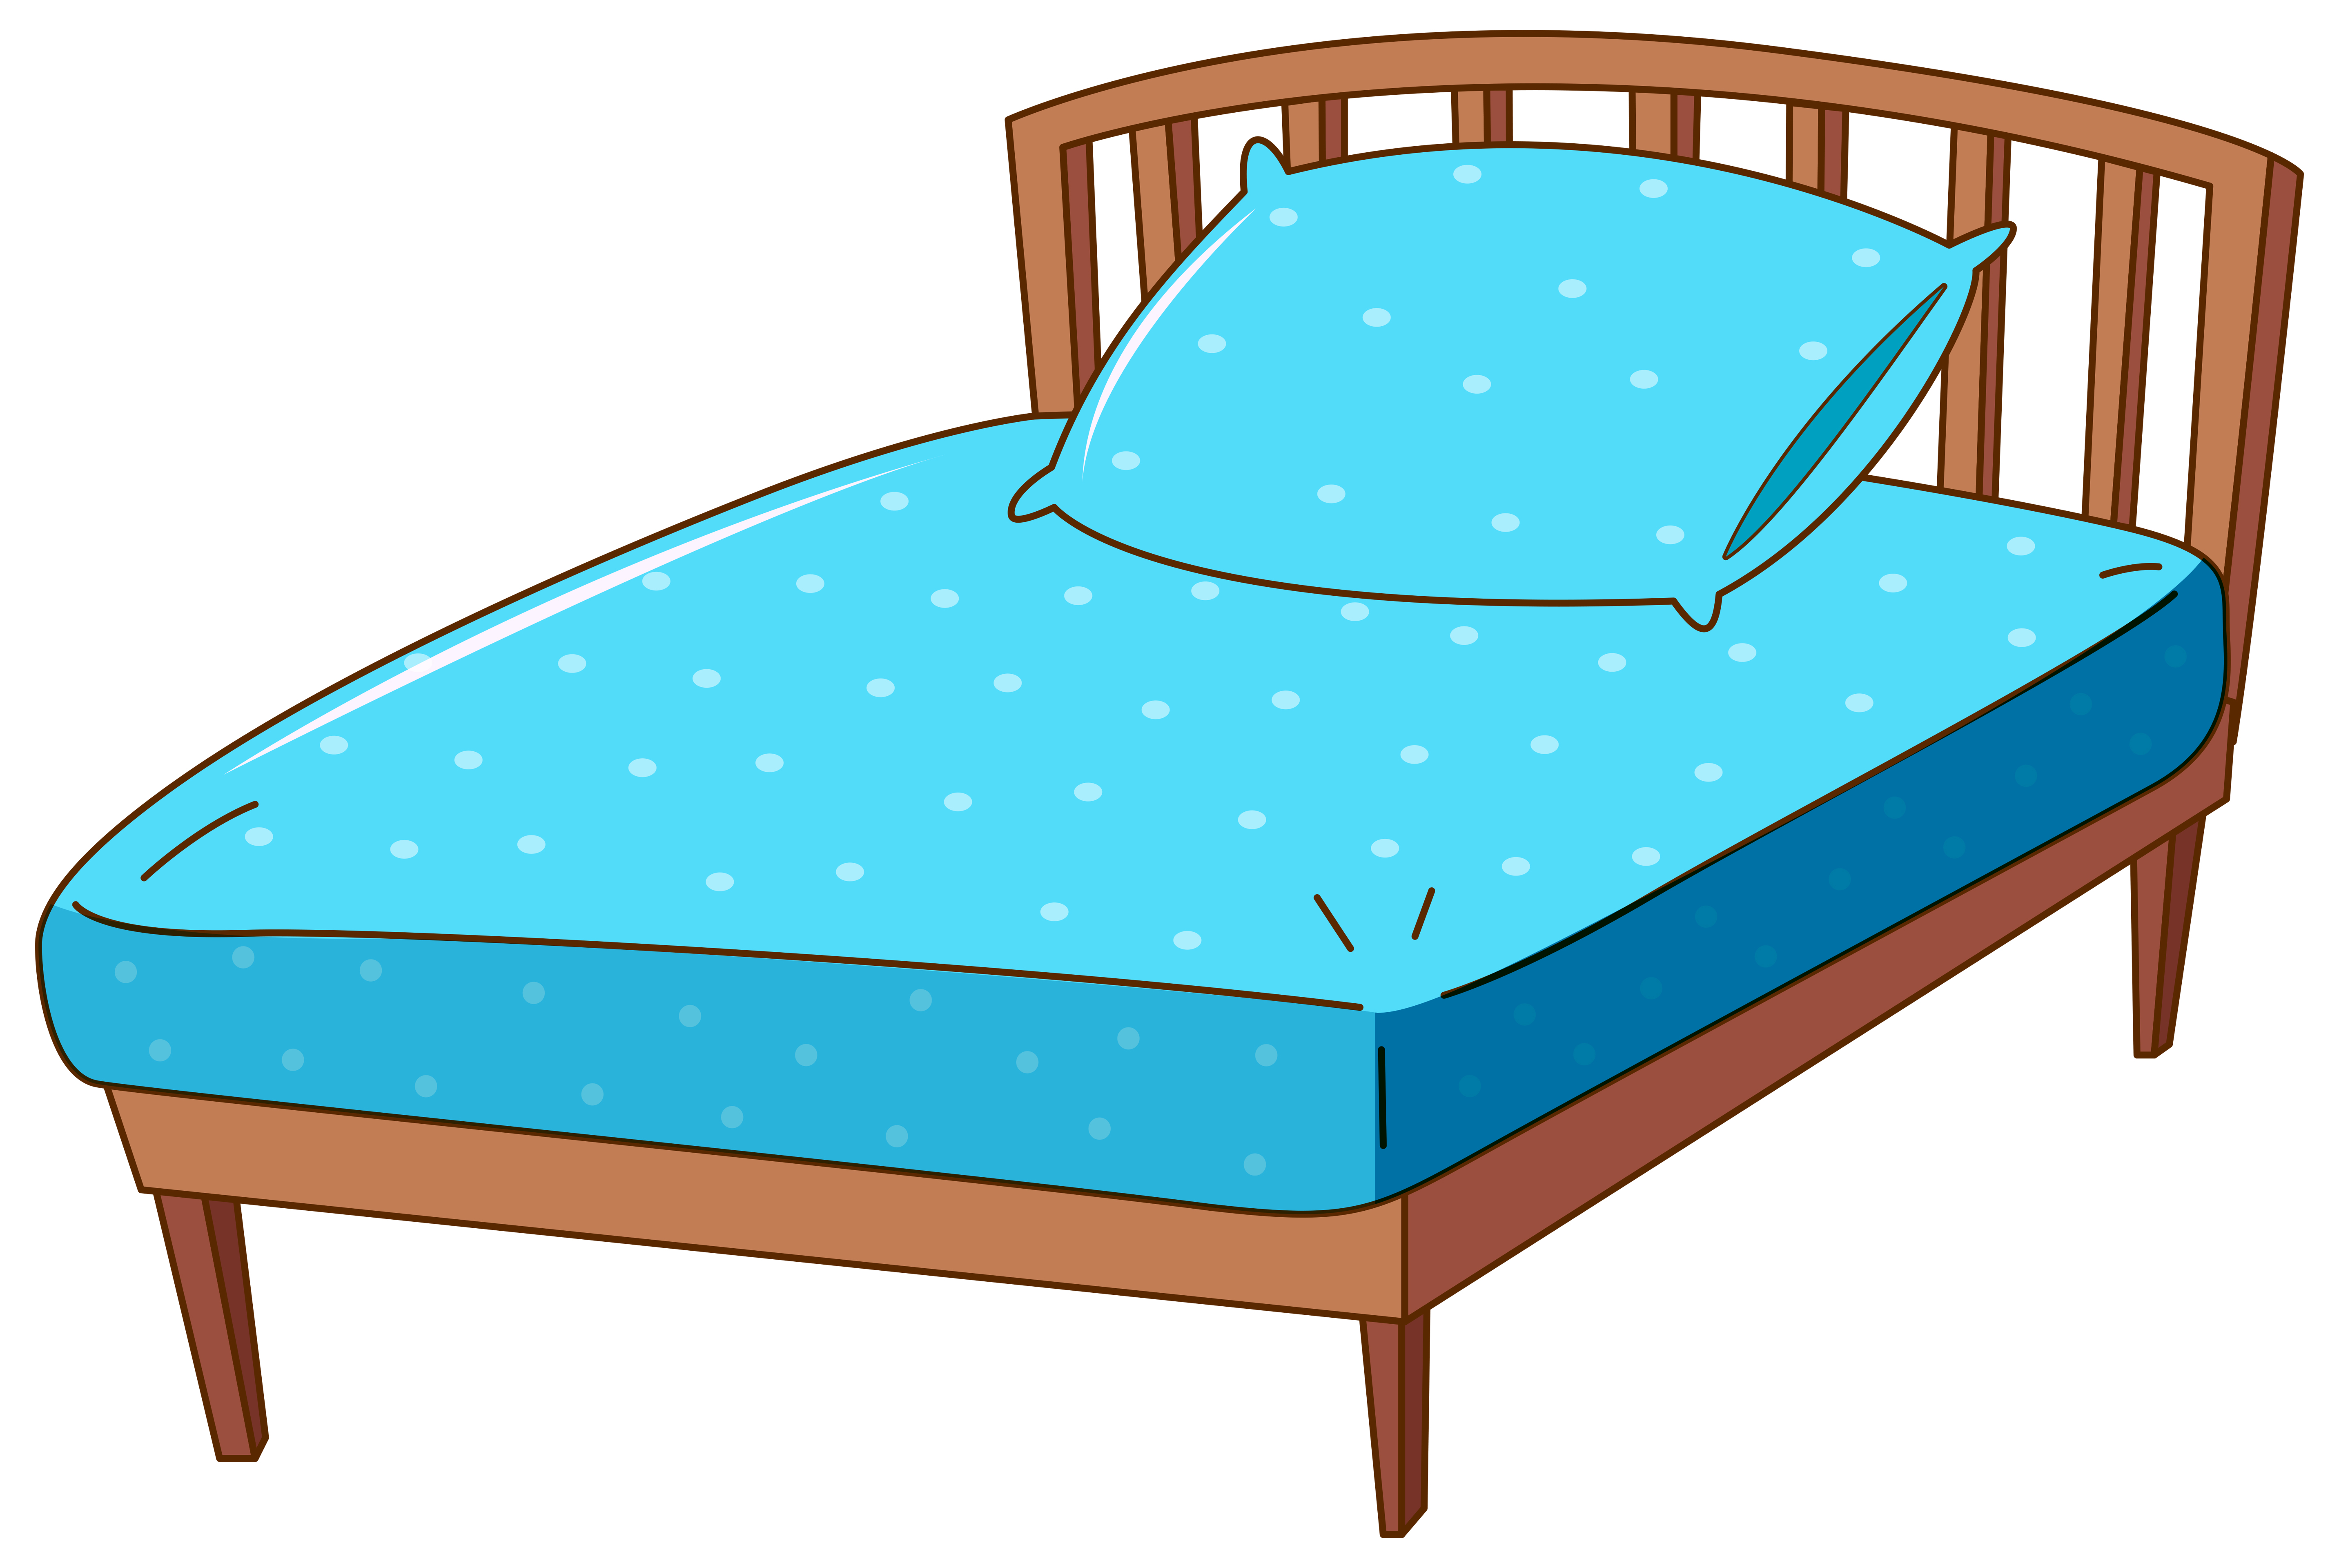
\includegraphics[width=.6\textwidth]{./media/image212.jpg}
\end{figure}

A PALAVRA QUE SE INICIA COM A MESMA LETRA DO MÓVEL É

\begin{multicols}{2}
\begin{escolha}

\item TELEFONE.

\item DADO.

\item CENOURA.

\item BARCO.
\end{escolha}
\end{multicols}

\num{4} VEJA ALIMENTO PREFERIDO DO RATINHO FIFI.

\begin{figure}[H]
\centering
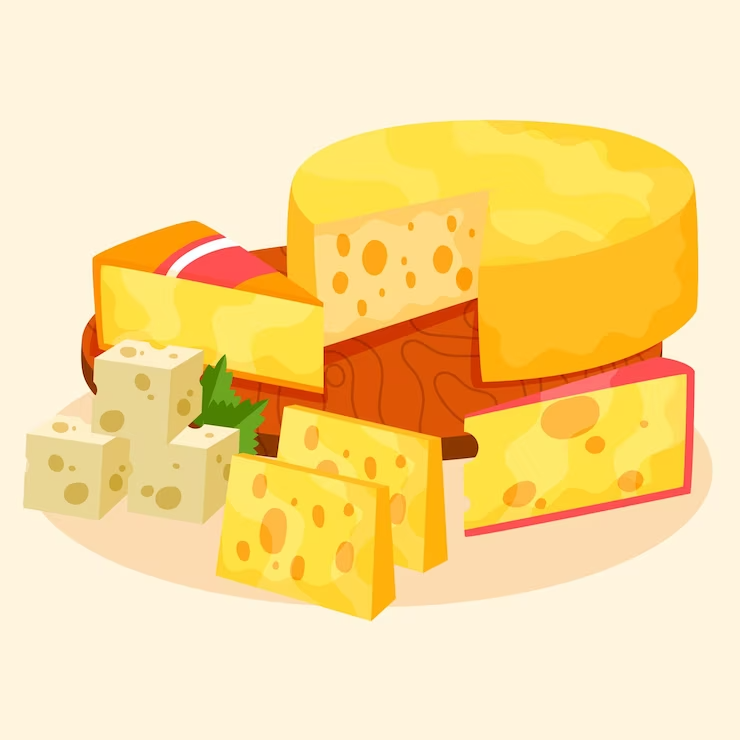
\includegraphics[width=.5\textwidth]{./media/image213.png}
\end{figure}

A ESCRITA CORRETA DO NOME DO ALIMENTO DE FIFI É

\begin{multicols}{2}
\begin{escolha}

\item QEIJO.

\item CUEIJO.

\item QUEIJO.

\item CUIJO.
\end{escolha}
\end{multicols}

\num{5} OBSERVE O ANIMAL PREFERIDO DE GUSTAVO.

\begin{figure}[H]
\centering

\includegraphics[width=.5\textwidth]{./media/image214.png}
\end{figure}

A SEPARAÇÃO SILÁBICA DO NOME DO ANIMAL É

\begin{escolha}

\item O – VE - LHA.

\item O- V- E-LHA.

\item O-VE- L- HA.

\item OVE- LH- A.

\end{escolha}

\num{6} OBSERVE A FRUTA FAVORITA DE FELIPE.

\begin{minipage}{.5\textwidth}
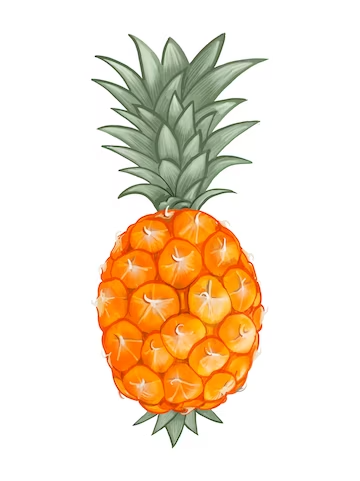
\includegraphics[width=.8\textwidth]{./media/image215.png}
\end{minipage}
\hspace{.5cm}
\begin{minipage}{.5\textwidth}
A FRUTA QUE SE INICIA COM A MESMA VOGAL INICIAL DA FRUTA FAVORITA DE FELIPE É

\begin{escolha}

\item GOIABA.

\item BANANA.

\item ABACATE.

\item GRAVIOLA.

\end{escolha}
\end{minipage}

\num{7} VEJA O BRINQUEDO QUE ARTHUR GANHOU EM UM SORTEIO:

\begin{figure}[H]
\centering
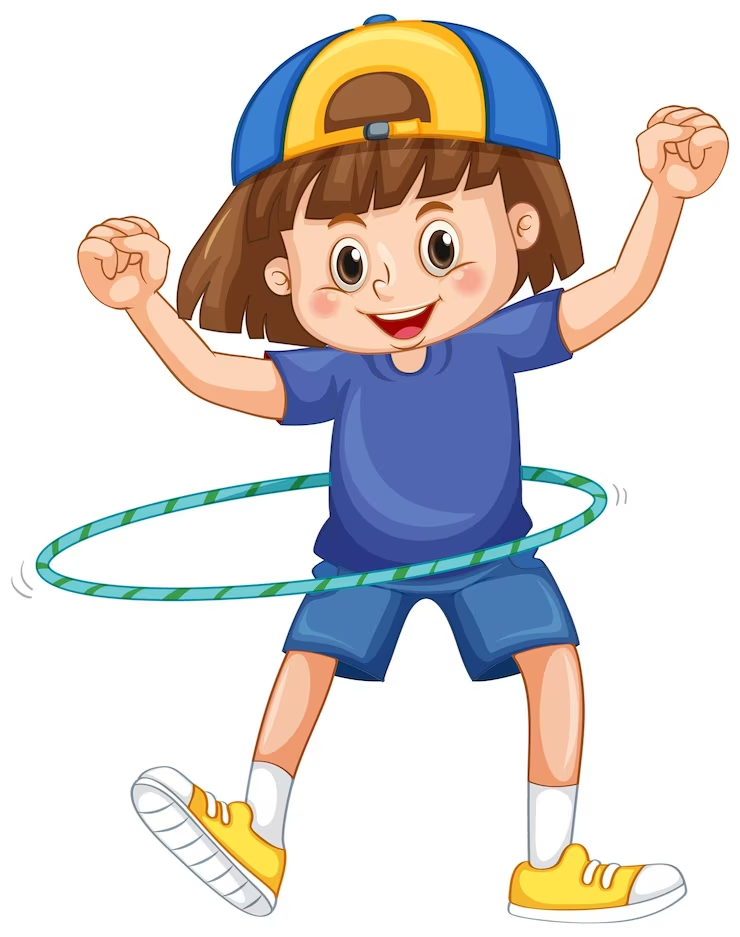
\includegraphics[width=.4\textwidth]{./media/image216.png}
\end{figure}

A PALAVRA CUJA SÍLABA INICIAL TAMBÉM APRESENTA O ESQUEMA CVC É

\begin{multicols}{2}
\begin{escolha}
\item PEDRA.

\item BATATA.

\item MORANGO.

\item COMPUTADOR.
\end{escolha}
\end{multicols}

\num{8} OBSERVE A IMAGEM A SEGUIR:

\begin{figure}[H]
\centering
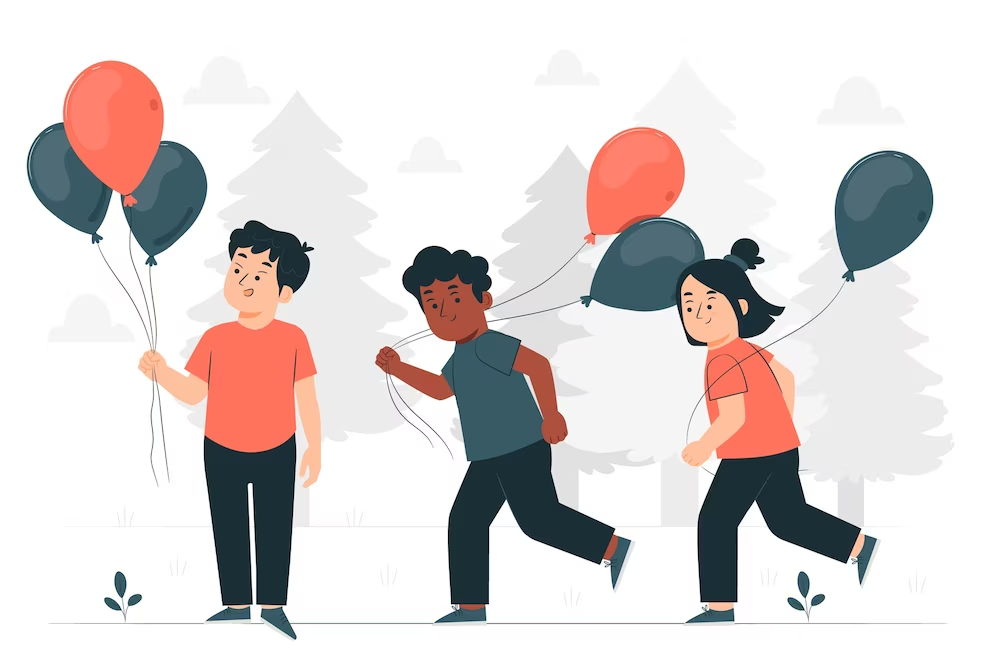
\includegraphics[width=.9\textwidth]{./media/image217.png}
\end{figure}

A FRASE QUE REPRESENTA A IMAGEM É

\begin{escolha}

\item AS CRIANÇAS BRINCAM COM BALÕES.

\item AS CRIANÇAS BRINCAM DE PIPA.

\item A MENINA BRINCA COM O PIÃO.

\item OS BALÕES DAS CRIANÇAS SUMIRAM.

\end{escolha}

\num{9} LEIA O TEXTO A SEGUIR.

\begin{myquote}
\textbf{A BARATA}

\begin{verse}
A BARATA DIZ QUE TEM
SETE SAIAS DE FILÓ.
É MENTIRA DA BARATA
ELA TEM É UMA SÓ.
AH! AH! AH!
OH! OH! OH!
ELA TEM É UMA SÓ.
A BARATA DIZ QUE TEM
SETE SAIAS DE BALÃO.
É MENTIRA ELA NÃO TEM
NEM DINHEIRO PRO SABÃO.
AH! AH! AH!
OH! OH! OH!
NEM DINHEIRO PRO SABÃO.
A BARATA DIZ QUE TEM
UM SAPATO DE FIVELA.
É MENTIRA DA BARATA
O SAPATO É DA MÃE DELA.
AH! AH! AH!
OH! OH! OH!
O SAPATO É DA MÃE DELA.
\end{verse}

\fonte{http://www.dominiopublico.gov.br/download/texto/me000588.pdf. Acesso 08 Mar 2023.}
\end{myquote}

O QUE A BARATA TEM EM APENAS UMA QUANTIDADE?

\begin{escolha}

\item SAIA DE FILÓ

\item SAIA DE BALÃO.

\item SAPATO DE FIVELA.

\item DINHEIRO PRA SABÃO.

\end{escolha}

\num{10} BIANCA VAI FAZER UM BOLO DE MILHO PARA RECEBER SUA AMIGA:

O TEXTO QUE ELA DEVE USAR É

\begin{escolha}

\item AGENDA.

\item CONVITE.

\item VERBETE.

\item RECEITA.

\end{escolha}

\num{11} LEIA O ANÚNCIO.

\begin{figure}[H]
\centering
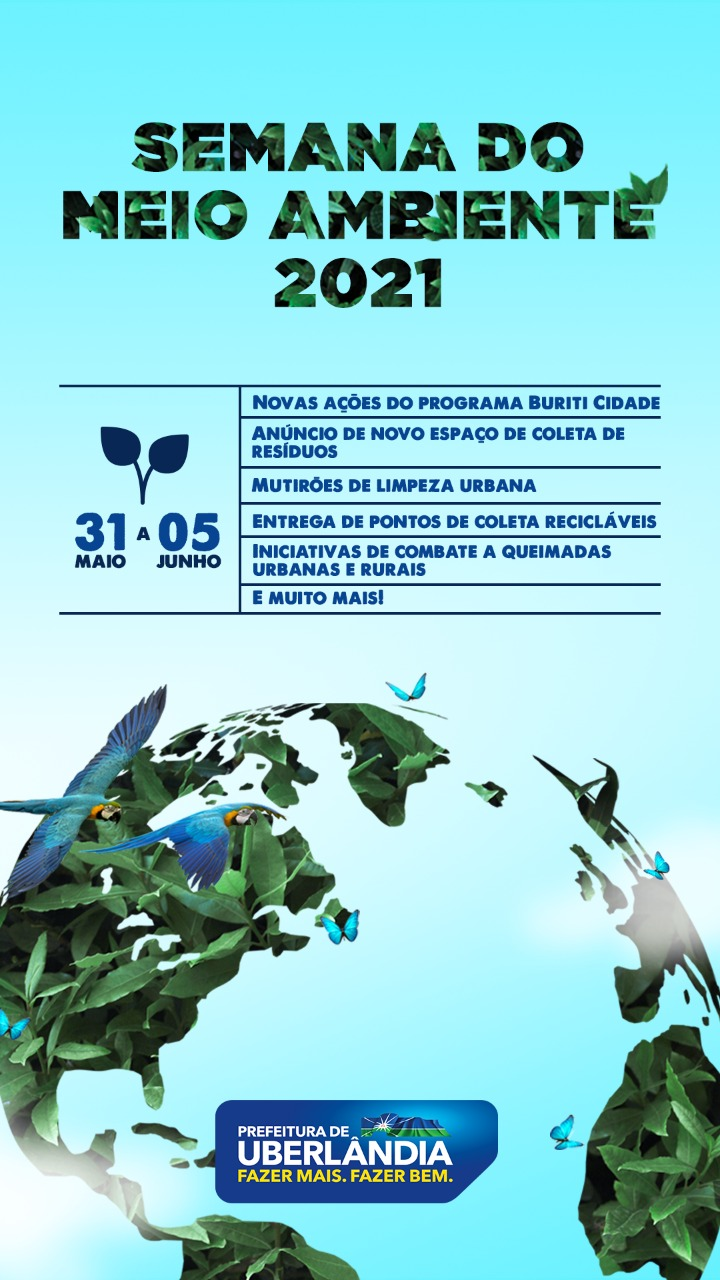
\includegraphics[width=.6\textwidth]{./media/image218.jpeg}
\end{figure}

ESSE TEXTO SERVE PARA

\begin{escolha}

\item ENSINAR.

\item DIVERTIR.

\item INFORMAR.

\item ANUNCIAR.

\end{escolha}

\pagebreak
\num{12} LEIA O TEXTO A SEGUIR.

\begin{myquote}
\textbf{SE ESTA RUA FOSSE MINHA}

\begin{verse}
SE ESTA RUA, SE ESTA RUA
FOSSE MINHA
EU MANDAVA,
EU MANDAVA LADRILHAR
COM PEDRINHAS,
COM PEDRINHAS DE BRILHANTES
PARA O MEU,
PARA O MEU AMOR PASSAR.
\end{verse}

\fonte{http://www.dominiopublico.gov.br/download/texto/me000588.pdf. Acesso 08 Mar 2023.}
\end{myquote}

POR QUE A RUA SERIA LADRILHADA?

\begin{escolha}

\item PORQUE ELA ERA DE OUTRA PESSOA.

\item PARA O MEU AMOR PASSAR.

\item PORQUE ELA ESTAVA QUEBRADA.

\item PORQUE ACONTECERIA UMA FESTA.

\end{escolha}

\num{13} LEIA O TEXTO A SEGUIR.

\begin{myquote}
\begin{verse}
MEIO-DIA
MACACO ASSOBIA
PANELA NO FOGO
BARRIGA VAZIA.
\end{verse}
\end{myquote}

A BARRIGA ESTÁ VAZIA PORQUE

\begin{escolha}

\item O FOGO TINHA APAGADO.

\item A COMIDA QUEIMOU NA PANELA.

\item O MACACO TINHA COMIDO TUDO.

\item A COMIDA ESTAVA SENDO PREPARADA.

\end{escolha}

\pagebreak
\num{14} OBSERVE A IMAGEM A SEGUIR.

\begin{figure}[H]
\centering
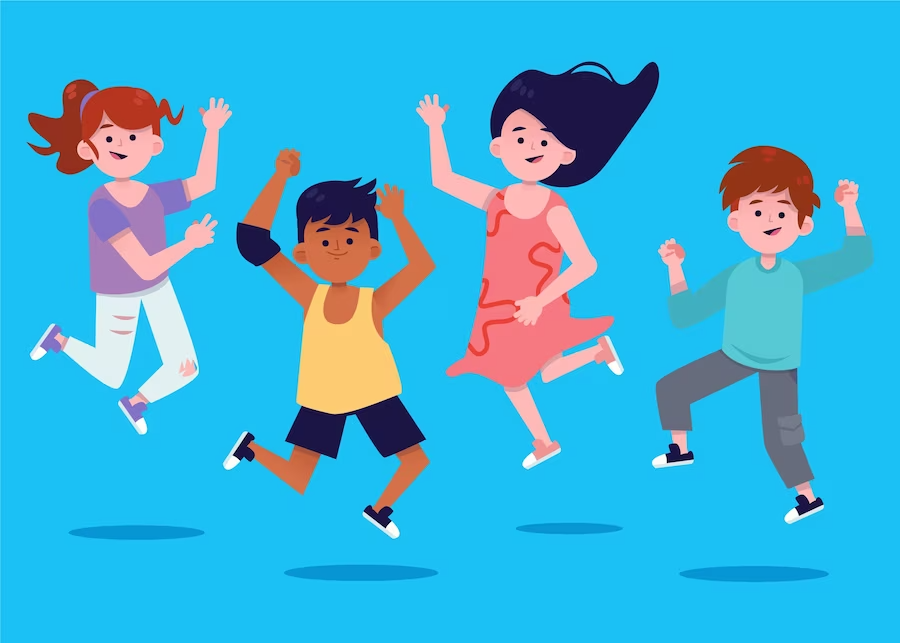
\includegraphics[width=.5\textwidth]{./media/image219.png}
\end{figure}

AS CRIANÇAS ESTÃO

\begin{multicols}{2}
\begin{escolha}

\item ANIMADAS.

\item TRISTES.

\item BRAVAS.

\item DORMINDO.

\end{escolha}
\end{multicols}

\num{15} OBSERVE A IMAGEM A SEGUIR.

\begin{figure}[H]
\centering

\includegraphics[width=.5\textwidth]{./media/image220.png}
\end{figure}

A EXPRESSÃO FACIAL DO GAROTO INDICA QUE ELE ESTÁ

\begin{escolha}

\item BRAVO.

\item TRISTE.

\item FELIZ.

\item CONFUSO.

\end{escolha}

\chapter[Simulado 2]{Simulado}
\markboth{Simulado 2}{}

\num{1} OBSERVE O PRESENTE QUE ANA GANHOU DA SUA MADRINHA.

\begin{figure}[H]
\centering
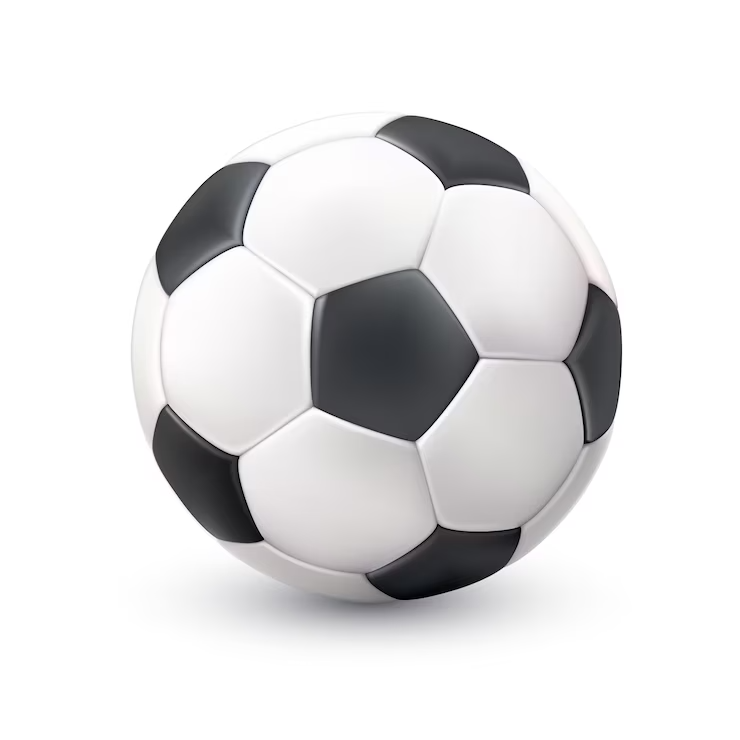
\includegraphics[width=.35\textwidth]{./media/image221.png}
\end{figure}

A PALAVRA CUJA LETRA INICIAL É A MESMA DO PRESENTE É

\begin{escolha}
\item PANELA.

\item BONECA.

\item VACINA.

\item FIGO

\end{escolha}

\num{2} OBSERVE A IMAGEM A SEGUIR.

\begin{figure}[H]
\centering

\includegraphics[width=.4\textwidth]{./media/image222.png}
\end{figure}

A PALAVRA QUE APRESENTA A MESMA SÍLABA INICIAL DO NOME DESSE ANIMAL É

\begin{escolha}
\item VALE.

\item FADA.

\item TOCA

\item PATO.

\end{escolha}

\num{3} VEJA O ALIMENTO QUE O COELHINHO PITOCO GOSTA DE COMER.

\begin{figure}[H]
\centering
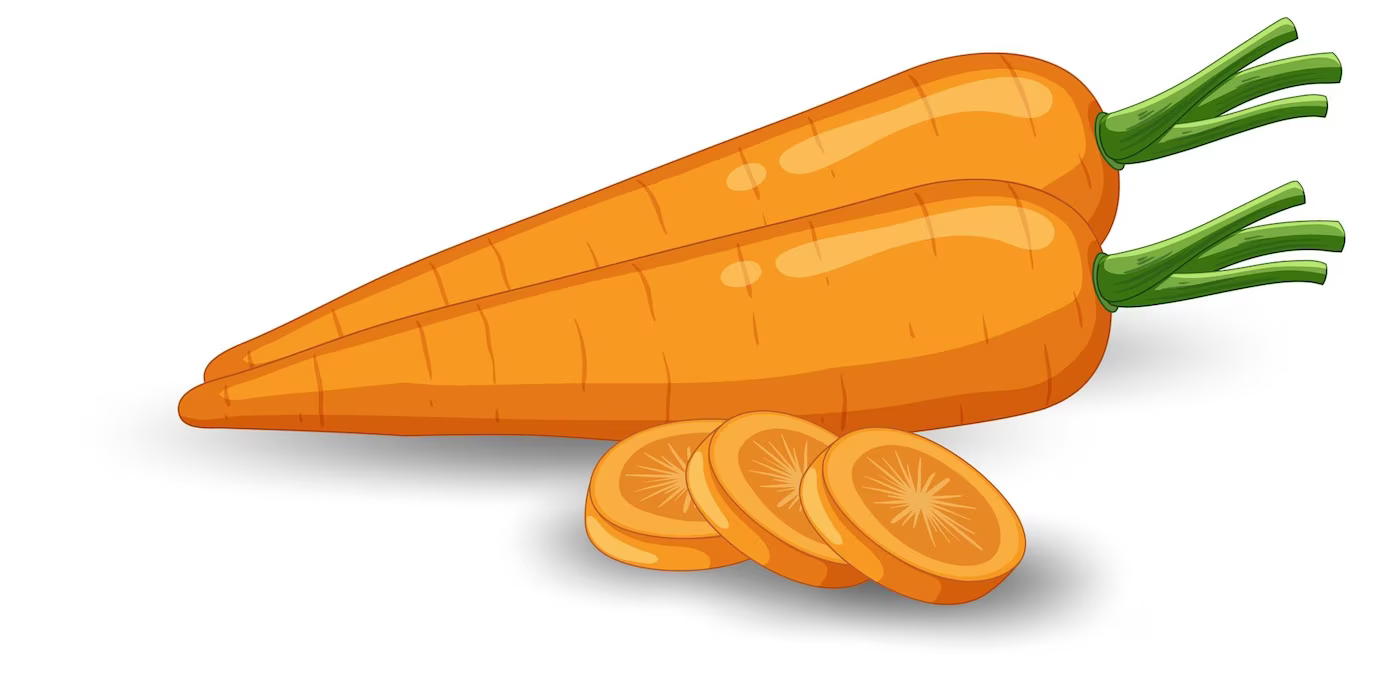
\includegraphics[width=\textwidth]{./media/image223.png}
\end{figure}

A PALAVRA QUE COMEÇA COM A MESMA SÍLABA DO NOME DO ALIMENTO DE PITOCO É

\begin{escolha}
\item CAMA.

\item COLA.

\item CEREJA.

\item CUSCUS.

\end{escolha}

\num{4} VEJA A PALAVRA QUE PEDRO E TIAGO FORMARAM NO JOGO DA FORCA.

\begin{myquote}
\begin{center}
\textbf{POMBA}
\end{center}
\end{myquote}

QUAL LETRA PODEMOS COLOCAR NA PRIMEIRA POSIÇÃO DA PALAVRA PARA FORMAR UMA OUTRA?

\begin{escolha}
\item D

\item B

\item F

\item V

\end{escolha}

\num{5} VEJA A PALAVRA QUE HUGO ESCREVEU.

\begin{myquote}
\begin{center}
\textbf{AMORA}
\end{center}
\end{myquote}

A SEPARAÇÃO SILÁBICA DO NOME QUE HUGO ESCREVEU É

\begin{escolha}

\item A - MO – RA.

\item AM - O – RA.

\item A - MO – R-A.

\item AMO- R - A.

\end{escolha}

\num{6} VEJA O PRESENTE QUE JONAS DEU PARA SUA AMIGA ELIZABETH

\begin{figure}[H]
\centering

\includegraphics[width=.6\textwidth]{./media/image224.png}
\end{figure}

QUAL PALAVRA APRESENTA A SÍLABA INICIAL FORMADA APENAS POR UMA VOGAL ASSIM COMO O NOME DO PRESENTE?

\begin{escolha}

\item BALA.

\item APITO.

\item ARVORE.

\item PANELA.

\end{escolha}

\num{7} OBSERVE A FRUTA QUE MARIA GOSTA DE LEVAR NA LANCHEIRA.

\begin{figure}[H]
\centering

\includegraphics[width=.5\textwidth]{./media/image74.png}
\end{figure}

A PALAVRA COM A SÍLABA MEDIAL FORMADA POR CONSOANTE-VOGAL-CONSOANTE, ASSIM COMO O NOME DA FRUTA DE QUE MARIA GOSTA, É 

\begin{escolha}

\item MELANCIA.

\item FORMIGA.

\item MOQUECA.

\item BATOM.

\end{escolha}

\num{8} MATEUS FOI AO HOSPITAL COM SUA MÃE E VIU ESSE CARRO NO LOCAL.

\begin{figure}[H]
\centering
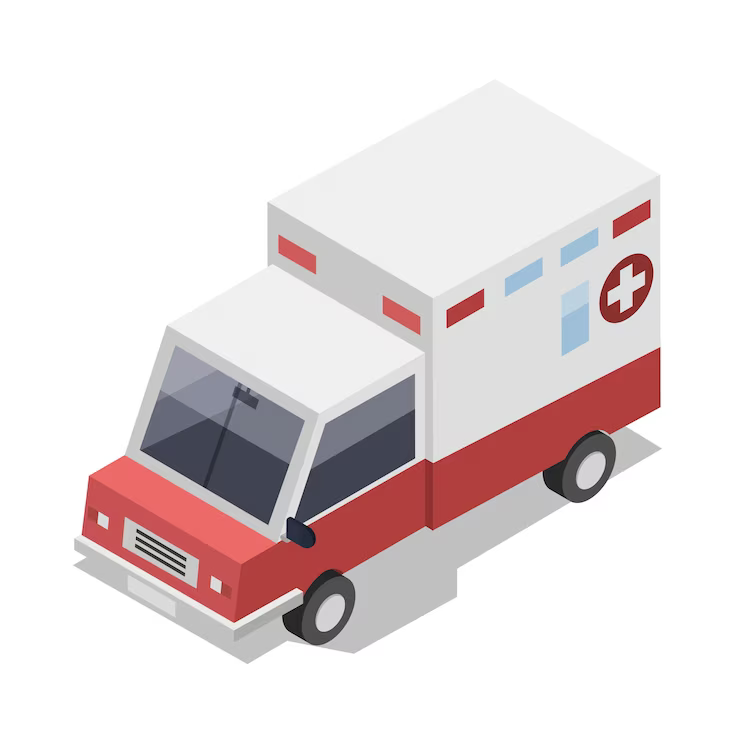
\includegraphics[width=\textwidth]{./media/image225.png}
\end{figure}

A ESCRITA CORRETA DO NOME DO CARRO É

\begin{escolha}

\item ABULÂNCIA.

\item AMBULÂCIA.

\item AMBULÂMCIA.

\item AMBULÂNCIA.

\end{escolha}

\pagebreak
\num{9} OBSERVE A IMAGEM A SEGUIR.

\begin{figure}[H]
\centering
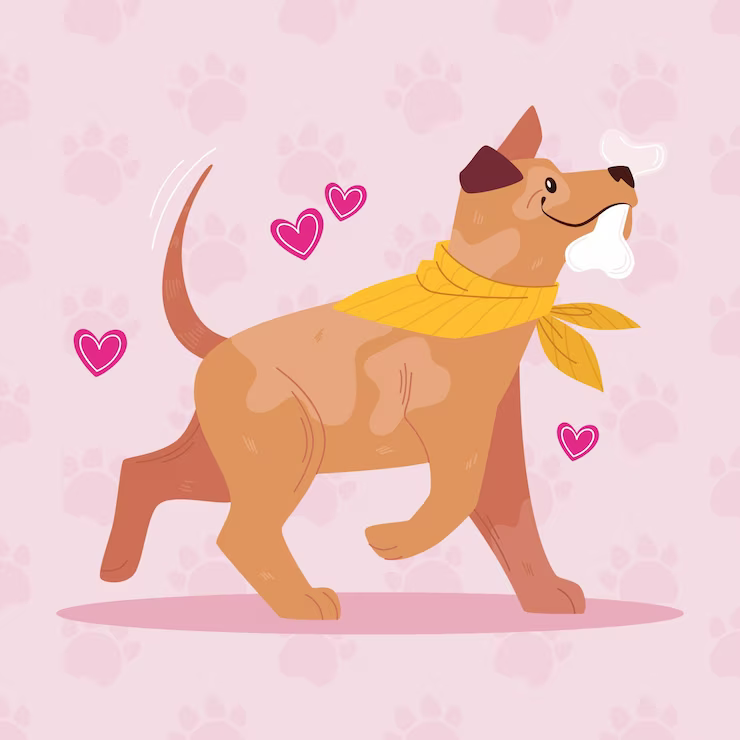
\includegraphics[width=.5\textwidth]{./media/image226.png}
\end{figure}

A PARTIR DA ILUSTRAÇÃO, PODEMOS DIZER QUE O CACHORRINHO ESTÁ FELIZ PORQUE

\begin{escolha}

\item ESTÁ BRINCANDO COM UM DISCO.

\item GANHOU UM OSSO.

\item ESTÁ BRINCANDO COM AS CRIANÇAS.

\item ESTÁ COMENDO RAÇÃO.

\end{escolha}

\num{10} OBSERVE A IMAGEM A SEGUIR.

\begin{figure}[H]
\centering

\includegraphics[width=.5\textwidth]{./media/image227.png}
\end{figure}

A FRASE QUE REPRESENTA A IMAGEM É

\begin{escolha}

\item O GATO PERSEGUE O CACHORRO.
\item O CACHORO LATE COM O GATO.
\item O CACHORRO E O GATO ESTÃO BRIGANDO.
\item O GATO E O CACHORROM ESTÃO BRINCANDO.

\end{escolha}

\num{11} LEIA O TEXTO A SEGUIR.

\begin{myquote}
\textbf{O ROUXINOL DO IMPERADOR}

O PALÁCIO DO IMPERADOR DA CHINA ERA UMA DAS COISAS MAIS
BONITAS QUE EXISTIAM NO MUNDO. CONSTRUÍDO EM MÁRMORE
BRANCO, POSSUÍA TORRES DE MARFIM, PAREDES REVESTIDAS COM
TECIDOS DE CORES VARIADAS E QUARTOS DECORADOS COM OURO E
PRATA. ERA REALMENTE UMA MARAVILHA!
O JARDIM TAMBÉM ERA DE ENORME BELEZA; NELE CRESCIAM
FLORES RARAS E BELAS. HAVIA INÚMEROS RIOS E LAGOS, ONDE
NADAVAM PEIXES DE TODAS AS ESPÉCIES E TAMANHOS.
PARA ALÉM DO JARDIM, SE ESTENDIA UMA MATA, QUE
CHEGAVA ATÉ O MAR E NO INTERIOR DELA VIVIA UM ROUXINOL DE
CANTO ÚNICO.

\fonte{http://www.dominiopublico.gov.br/download/texto/me001614.pdf. Acesso em 10 Mar 2023.}
\end{myquote}

ONDE VIVIA O ROUXINOL?

\begin{escolha}

\item NA MATA.

\item NO JARDIM.

\item NAS FLORES.

\item NO PALÁCIO. 

\end{escolha}

\num{12} OBSERVE O CARTAZ A SEGUIR.

\begin{figure}[H]
\centering

\includegraphics[width=.6\textwidth]{./media/image228.png}
\end{figure}

ONDE É COMUM VER ESSE TIPO DE CARTAZ?

\begin{escolha}

\item NAS IGREJAS.

\item NAS FAZENDAS.

\item NOS LOCAIS PÚBLICOS.

\item NOS HOSPITAIS PARTICULARES.

\end{escolha}

\num{13} LEIA O TEXTO A SEGUIR.

\begin{myquote}
\textbf{O LOBO E O CÃO}

UM LOBO E UM CÃO SE ENCONTRARAM NUM CAMINHO. DISSE O LOBO: — COMPANHEIRO, VOCÊ ESTÁ COM ÓTIMO ASPECTO: GORDO, O PÊLO LUSTROSO... ESTOU ATÉ COM INVEJA! — ORA, FAÇA COMO EU — RESPONDEU O CÃO. — ARRANJE UM BOM AMO. EU TENHO COMIDA NA HORA CERTA, SOU BEM TRATADO... MINHA ÚNICA OBRIGAÇÃO É LATIR À NOITE, QUANDO APARECEM LADRÕES. 

\fonte{http://www.dominiopublico.gov.br/download/texto/me001614.pdf. Acesso em 10 Mar 2023.}
\end{myquote}

O ASSUNTO DO TEXTO É

\begin{escolha}

\item A INVEJA DO LOBO PELO CÃO.

\item A DESPEDIDA DO LOBO E O CÃO.

\item O ENCONTRO DO CÃO E O LOBO.

\item O CONVITE QUE O CÃO FEZ PARA O LOBO.

\end{escolha}

\num{14} LEIA O TEXTO A SEGUIR.

\begin{myquote}
\begin{verse}
LÁ VAI A BOLA
GIRAR NA RODA
PASSEAR DEPRESSA
E SEM DEMORA
E SE NO FIM
DESTA CANÇÃO
VOCÊ ESTIVER
COM A BOLA NA MÃO
DEPRESSA PULE FORA.
\end{verse}

\fonte{http://www.dominiopublico.gov.br/download/texto/me000588.pdf. Acesso 12 Mar 2023.}
\end{myquote}

\pagebreak
O QUE ACONTECE COM QUEM FICAR COM A BOLA NA MÃO?

\begin{escolha}

\item SAI DA BRINCADEIRA.
\item PULA DE UM PÉ SÓ.
\item GIRA NA RODA.
\item GANHA A BOLA.

\end{escolha}

\num{15} OBSERVE A IMAGEM A SEGUIR.

\begin{figure}[H]
\centering

\includegraphics[width=.7\textwidth]{./media/image229.jpg}
\end{figure}

O QUE O GATINHO ESTÁ FAZENDO?

\begin{escolha}

\item ESTÁ DORMINDO.

\item ESTÁ CORRENDO.

\item ESTÁ BRINCANDO.

\item ESTÁ COMENDO.

\end{escolha}

\chapter[Simulado 3]{Simulado}
\markboth{Simulado 3}{}

\num{1} VEJA O MATERIAL ESCOLAR QUE MARCOS GANHOU DA SUA TIA.

\begin{figure}[H]
\centering

\includegraphics[width=.45\textwidth]{./media/image230.png}
\end{figure}

A PALAVRA QUE COMEÇA COM A MESMA LETRA INICIAL DO OBJETO QUE MARCOS GANHOU É

\begin{multicols}{2}
\begin{escolha}

\item FERRO.

\item TOMATE.

\item DOMINÓ.

\item VASSOURA.

\end{escolha}
\end{multicols}

\num{2} VEJA A PALAVRA QUE ANA ESCREVEU.

\begin{myquote}
\begin{center}
\textbf{VILA}
\end{center}
\end{myquote}

A PALAVRA QUE SE INICIA COM A MESMA SÍLABA DA PALAVRA QUE ELA ESCREVEU É

\begin{escolha}

\item FILA.

\item BALA.

\item VELA.

\item VIGA.

\end{escolha}

\num{3} VEJA O PÁSSARO QUE PAULA AVISTOU NA ÁRVORE.

\begin{figure}[H]
\centering
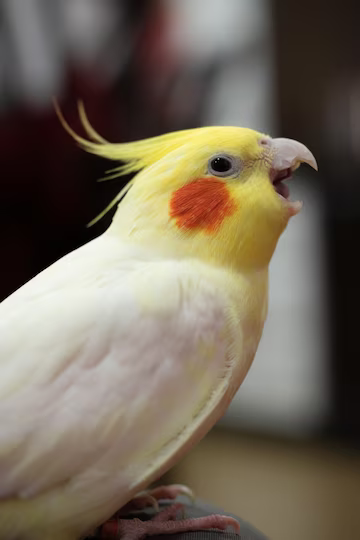
\includegraphics[width=.75\textwidth]{./media/image231.png}
\end{figure}

A ESCRITA CORRETA DO NOME DESSE PÁSSARO É

\begin{escolha}

\item PEREQUTO.

\item PERICUITO.

\item PERIQUITO.

\item PERIQITO.

\end{escolha}

\num{4} VEJA A PALAVRA QUE AS AMIGAS DESCOBRIRAM NO JOGO DA FORCA.

\begin{myquote}
\begin{center}
\textbf{CABELO}
\end{center}
\end{myquote}

A PALAVRA CUJA SOM INICIAL É O MESMO SOM DA PALAVRA QUE ELAS DESCOBRIRAM É

\begin{escolha}

\item CUSCUS.

\item CINEMA.

\item CEBOLA.

\item CISNE.

\end{escolha}

\num{5} VEJA A PALAVRA QUE LÍVIA LEU PARA SUA PROFESSORA.

\begin{myquote}
\begin{center}
\textbf{TAMANCO}
\end{center}
\end{myquote}

A PALAVRA CUJA SÍLABA MEDIAL TAMBÉM É FORMADA POR CONSOANTE-VOGAL-CONSOANTE É

\begin{escolha}

\item BANCO.

\item TAPETE.

\item MACACO.

\item MORANGO.

\end{escolha}

\num{6} OBSERVE A IMAGEM A SEGUIR.

\begin{figure}[H]
\centering

\includegraphics[width=.45\textwidth]{./media/image232.png}
\end{figure}

A ESCRITA CORRETA DO NOME DA FIGURA É

\begin{escolha}

\item BALAO

\item DALÃO

\item BALÃO

\item DALAÕ.

\end{escolha}

\num{7} VEJA O PRESENTE QUE TALITA GANHOU DA SUA AMIGA.

\begin{figure}[H]
\centering
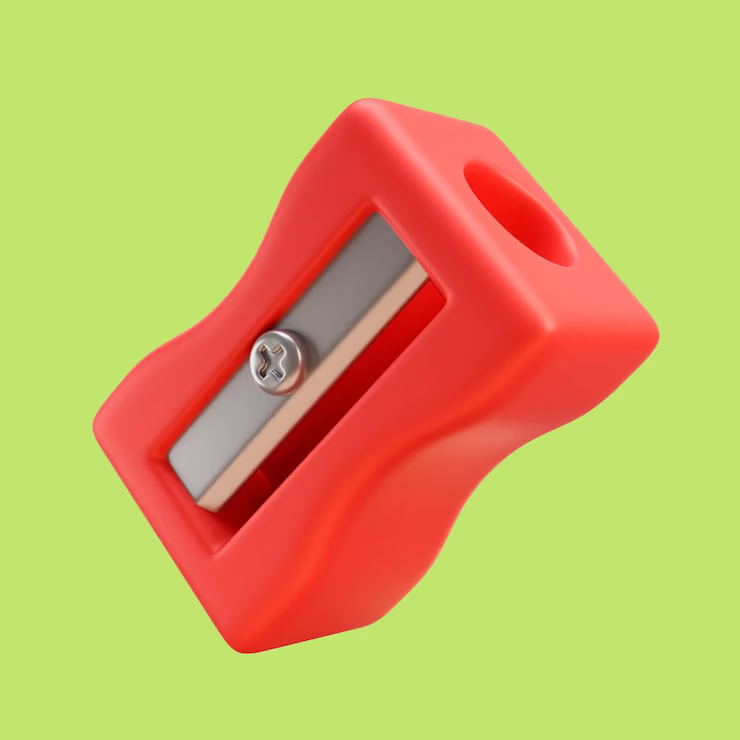
\includegraphics[width=.7\textwidth]{./media/image233.png}
\end{figure}

A SEPARAÇÃO SILÁBICA CORRETA DO NOME DA FIGURA É

\begin{escolha}

\item AP – ON – TA -DOR.

\item A - PON – TA - DOR.

\item APO - N- TA- DO -R.

\item A – PON -T-ADOR

\end{escolha}

\pagebreak
\num{8} OBSERVE A IMAGEM A SEGUIR.

\begin{figure}[H]
\centering
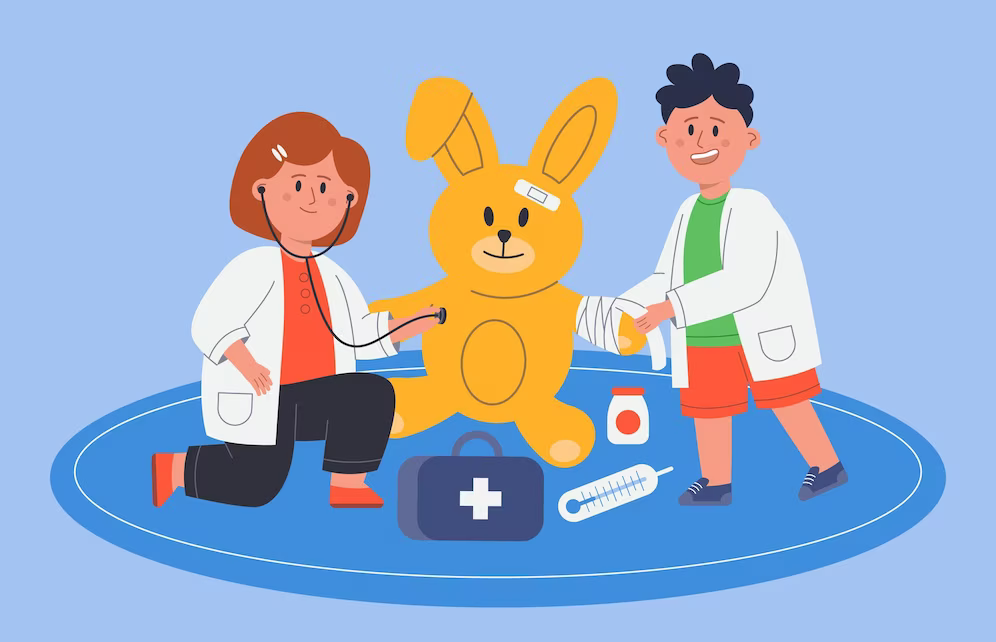
\includegraphics[width=.7\textwidth]{./media/image234.png}
\end{figure}

A SEPARAÇÃO SILÁBICA CORRETA DO NOME DA FIGURA É

\begin{escolha}

\item AS CRIANÇAS GOSTAM DO CACHORRO.

\item AS CRIANÇAS BRINCAM DE BONECA.

\item AS CRIANÇAS ESTÃO BRINCANDO DE HOSPITAL.

\item AS CRIANÇAS ESTÃO ANDANDO DE BICICLETA.

\end{escolha}

\num{9} LEIA O TEXTO A SEGUIR.

\begin{myquote}
\textbf{SALADA SAUDÁVEL}

INGREDIENTES:
1 PRATO RASO DE RÚCULA
1 PRATO RASO DE ALFACE AMERICANA 
1 PRATO RASO DE ALFACE ROXA
2 XÍCARAS DE TOMATE CEREJA
4 NOZES PICADAS
4 CASTANHAS DO BRASIL PICADAS 
6 DAMASCOS SECOS PICADOS
PREPARO:
MISTURAR TODOS OS INGREDIENTES EM UMA SALADEIRA E SERVIR.

\end{myquote}

QUANTOS DAMASCOS SERÃO USADOS PARA PREPARAR A RECEITA?

\begin{escolha}

\item UM.

\item DOIS.

\item SEIS.

\item QUATRO.

\end{escolha}

\num{10} MARTA VAI AO MERCADO FAZER AS COMPRAS DA SEMANA.
O TIPO DE TEXTO QUE ELA DEVERÁ USAR PARA ORGANIZAR OS ITENS DA COMPRA É

\begin{escolha}

\item LISTA.

\item AGENDA.

\item BILHETE.

\item ANÚNCIO.

\end{escolha}

\num{11} OBSERVE A IMAGEM A SEGUIR.

\begin{figure}[H]
\centering
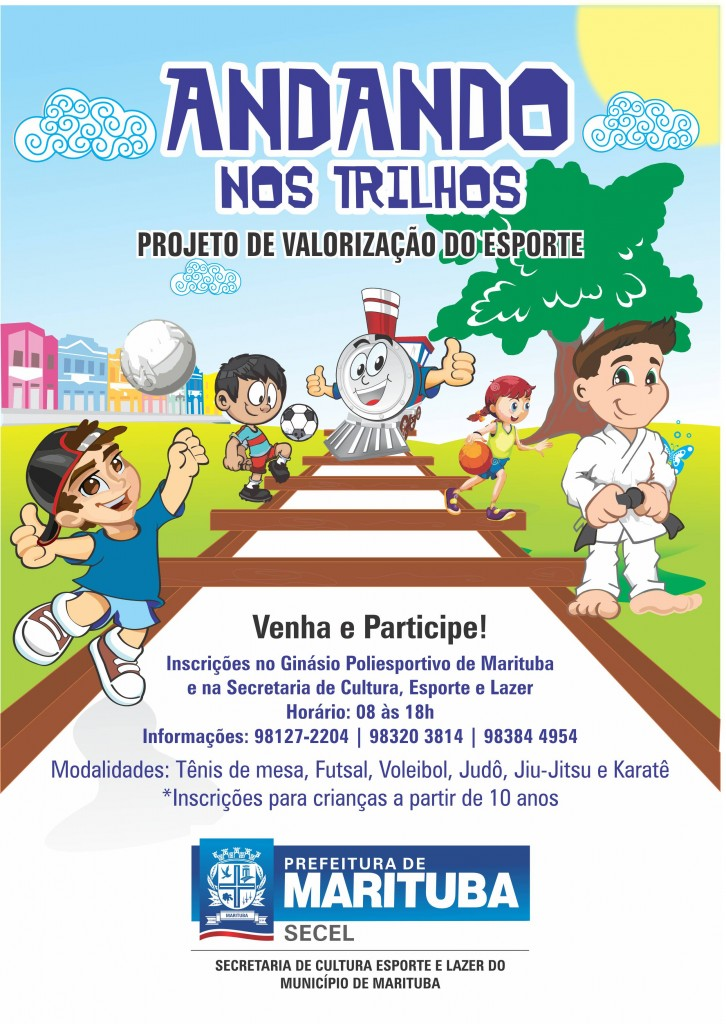
\includegraphics[width=.75\textwidth]{./media/image235.jpg}
\end{figure}

ESSE ANÚNCIO É DESTINADO A

\begin{escolha}

\item OS IDOSOS.

\item AS ADULTOS.

\item AS CRIANÇAS.

\item AS MULHERES.

\end{escolha}

\num{12} OBSERVE A IMAGEM A SEGUIR.

\begin{figure}[H]
\centering
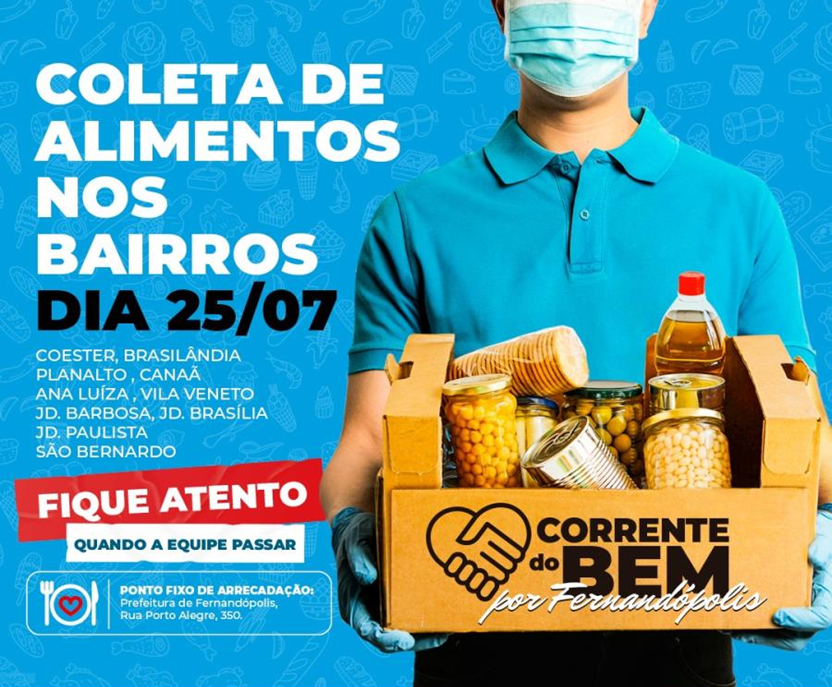
\includegraphics[width=.8\textwidth]{./media/image236.png}
\end{figure}

QUAL É O ASSUNTO DESSE TEXTO?

\begin{escolha}

\item VENDA DE ALIMENTOS.

\item DOAÇÃO DE ALIMENTOS.

\item COMPRA DE ALIMENTOS.

\item SELEÇÃO DE ALIMENTOS.

\end{escolha}

\pagebreak
\num{13} LEIA O TEXTO A SEGUIR.

\begin{myquote}
\textbf{O CORVO E O JARRO}

UM CORVO, QUASE MORTO DE SEDE, FOI A UM JARRO, ONDE PENSOU ENCONTRAR ÁGUA. QUANDO METEU O BICO PELA BORDA DO JARRO, VERIFICOU QUE SÓ HAVIA UM RESTINHO NO FUNDO. ERA DIFÍCIL ALCANÇÁ-LA COM O BICO, POIS O JARRO ERA MUITO ALTO.
DEPOIS DE VÁRIAS TENTATIVAS, PRECISOU DESISTIR, DESESPERADO. SURGIU, ENTÃO, UMA IDEIA EM SEU CÉREBRO.
APANHOU UMA PEDRA E JOGOU-A NO FUNDO DO JARRO. JOGOU MAIS
ALGUMAS E MUITAS OUTRAS.
COM ALEGRIA VERIFICOU QUE A ÁGUA VINHA, AOS POUCOS, SE APROXIMANDO DA BORDA. JOGOU MAIS ALGUMAS PEDRAS E CONSEGUIU MATAR A SEDE, SALVANDO SUA VIDA.

\fonte{http://www.dominiopublico.gov.br/download/texto/me001614.pdf. Acesso 12 Mar 2023.}
\end{myquote}

O TEXTO FALA DA

\begin{escolha}

\item INTELIGÊNCIA DO CORVO.

\item ALEGRIA DO CORVO.

\item JARRO DO CORVO.

\item SEDE DO CORVO.

\end{escolha}

\num{14} OBSERVE A IMAGEM A SEGUIR.

\begin{figure}[H]
\centering

\includegraphics[width=.5\textwidth]{./media/image237.png}
\end{figure}

\pagebreak
DE ACORDO COM SUA EXPRESSÃO FACIAL, O GAROTO ESTÁ

\begin{escolha}

\item TRISTE.

\item BRAVO.

\item DORMINDO.

\item FELIZ.

\end{escolha}

\num{15} LEIA O TEXTO A SEGUIR.

\begin{myquote}
\textbf{A FORMIGA E A POMBA}

UMA FORMIGA SEDENTA CHEGOU À MARGEM DO RIO, PARA BEBER
ÁGUA. PARA ALCANÇAR A ÁGUA, PRECISOU DESCER POR UMA FOLHA DE
GRAMA. AO FAZER ISSO, ESCORREGOU E CAIU DENTRO DA CORRENTEZA.
POUSADA NUMA ÁRVORE PRÓXIMA, UMA POMBA VIU A
FORMIGA EM PERIGO. RAPIDAMENTE, ARRANCOU UMA FOLHA DE
ÁRVORE E JOGOU DENTRO DO RIO, PERTO DA FORMIGA, QUE PÔDE SUBIR
NELA E FLUTUAR ATÉ A MARGEM.

\fonte{http://www.dominiopublico.gov.br/download/texto/me001614.pdf. Acesso em 12 Mar 2023.}
\end{myquote}

O TEXTO FALA DA

\begin{escolha}

\item AJUDAR A FORMIGA.

\item AFOGAR A FORMIGA.

\item ESPANTAR A FORMIGA.

\item ALIMENTAR A FORMIGA.

\end{escolha}

\chapter[Simulado 4]{Simulado}
\markboth{Simulado 4}{}

\num{1} VEJA O ANIMAL PREFERIDO DE JÚLIA.

\begin{figure}[H]
\centering
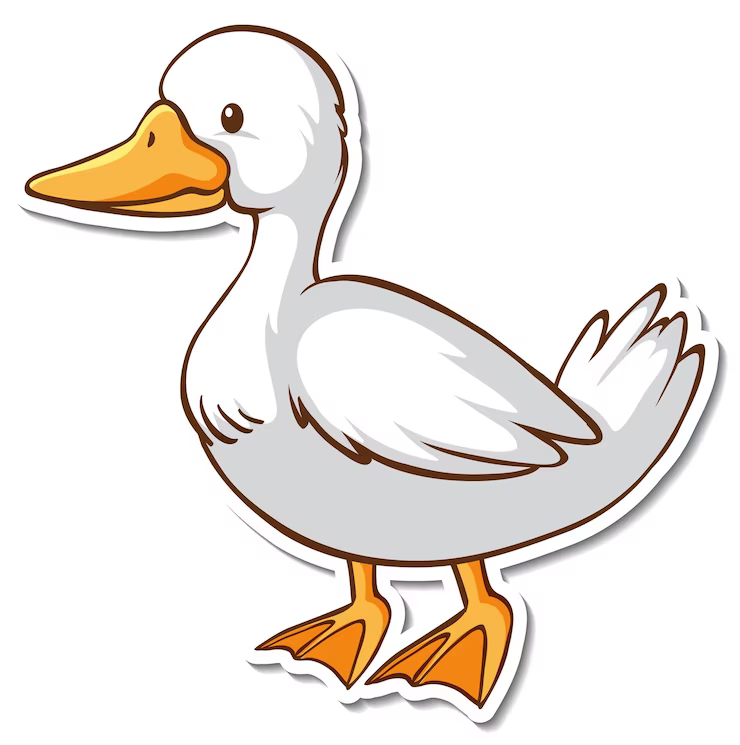
\includegraphics[width=.8\textwidth]{./media/image238.png}
\end{figure}

A PALAVRA CUJA LETRA INICIAL É A MESMA DO ANIMAL É

\begin{escolha}

\item VELA.

\item FAFÁ.

\item BALA.

\item PIPA.

\end{escolha}

\pagebreak
\num{2} VEJA A FRUTA QUE MARIA LEVARÁ AO PIQUENIQUE.

\begin{figure}[H]
\centering
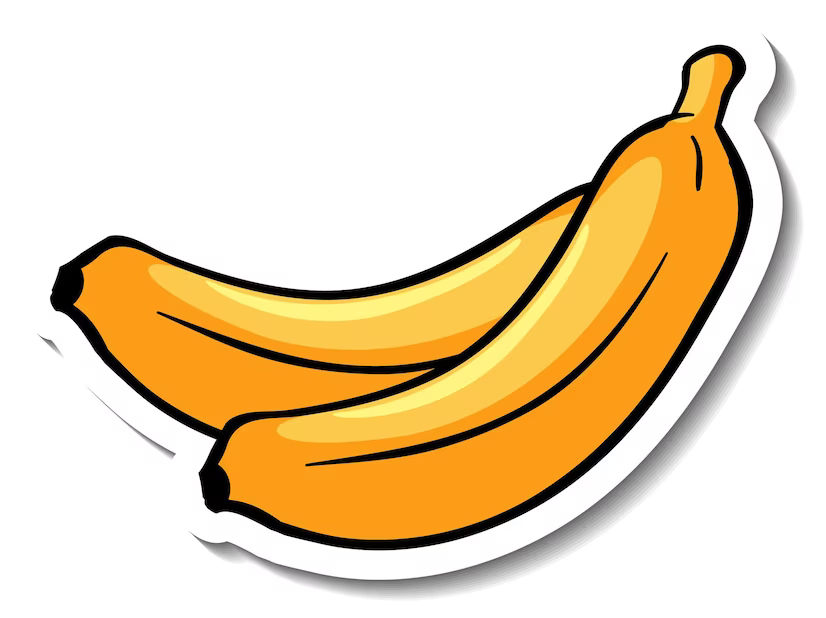
\includegraphics[width=.75\textwidth]{./media/image72.png}
\end{figure}

A PALAVRA QUE APRESENTA A MESMA SÍLABA INICIAL DA FRUTA É

\begin{escolha}

\item DADO.

\item BALA.

\item FADA.

\item PATO.

\end{escolha}

\num{3} VEJA O VEGETAL FAVORITO DE PAULA.

\begin{myquote}
\begin{center}
\textbf{CEBOLA}
\end{center}
\end{myquote}

A PALAVRA QUE APRESENTA A MESMA SÍLABA INICIAL DESSE VEGETAL É

\begin{escolha}

\item CINTO.

\item CUSCUS.

\item CERTO.

\item CARROÇA.

\end{escolha}

\pagebreak
\num{4} VEJA A PALAVRA QUE CARLA E MARIA FORMARAM NO ALFABETO MÓVEL.

\begin{myquote}
\begin{center}
\textbf{BANDA}
\end{center}
\end{myquote}

QUAL LETRA DEVE SER COLOCADA NA PRIMEIRA POSIÇÃO DA PALAVRA PARA FORMARMOS OUTRO TERMO?

\begin{escolha}

\item D

\item P

\item F

\item V

\end{escolha}

\num{5} OBSERVE O BRINQUEDO QUE THIAGO GANHOU.

\begin{figure}[H]
\centering
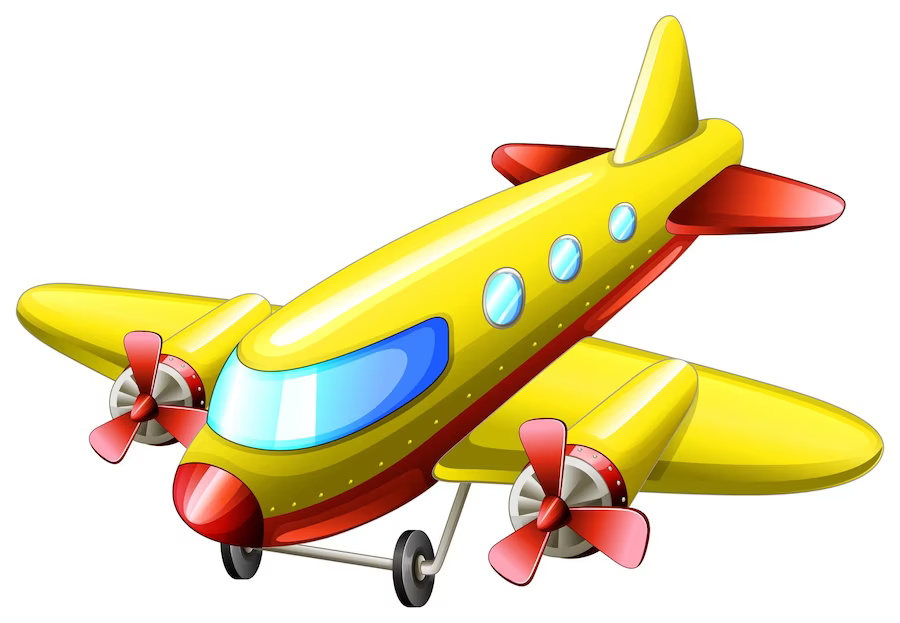
\includegraphics[width=.7\textwidth]{./media/image239.png}
\end{figure}

QUAL PALAVRA APRESENTA A SÍLABA INICIAL FORMADA APENAS POR VOGAL, ASSIM COMO O NOME DO BRINQUEDO QUE THIAGO GANHOU?

\begin{escolha}

\item FADA.

\item CRAVO.

\item ARMÁRIO.

\item ABACAXI.

\end{escolha}

\pagebreak
\num{6} VEJA A PALAVRA QUE ANA ESCREVEU.

\begin{myquote}
\begin{center}
\textbf{PEDRA}
\end{center}
\end{myquote}

QUAL PALAVRA TAMBÉM POSSUI A SÍLABA FINAL FORMADA POR CONSOANTE-VOGAL-CONSOANTE, ASSIM COMO ESSA PALAVRA?

\begin{escolha}

\item APITO.

\item CRAVO.

\item COMADRE. 

\item ESCRAVO.

\end{escolha}

\num{7} VEJA O OBJETO QUE A TIA DA MARIA COMPROU.

\begin{figure}[H]
\centering
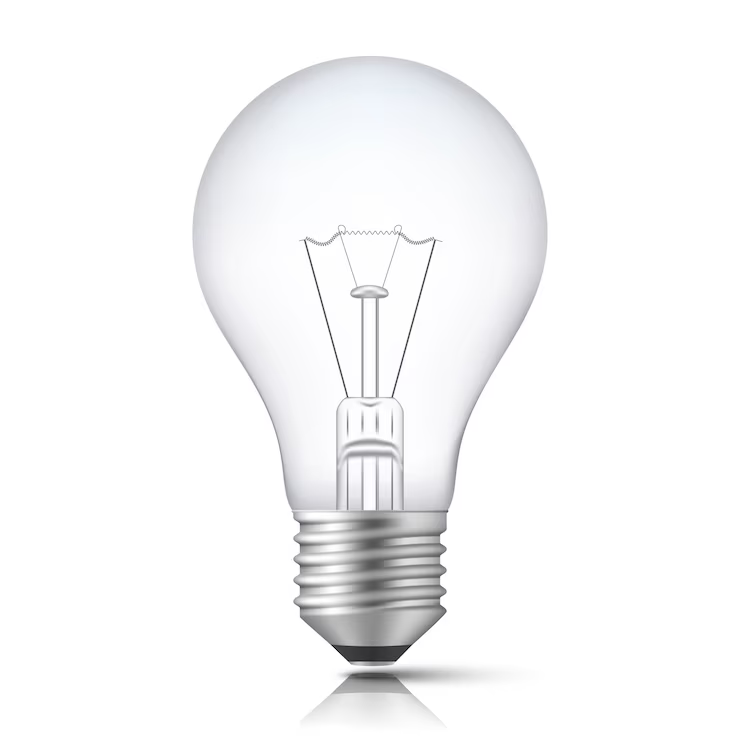
\includegraphics[width=.6\textwidth]{./media/image240.png}
\end{figure}

A ESCRITA CORRETA DO NOME DESSE OBJETO É

\begin{escolha}

\item LÂPADA.

\item LÂPAMDA.

\item LÂMPADA.

\item LÂNPADA.

\end{escolha}

\num{8} OBSERVE A IMAGEM A SEGUIR.

\begin{figure}[H]
\centering
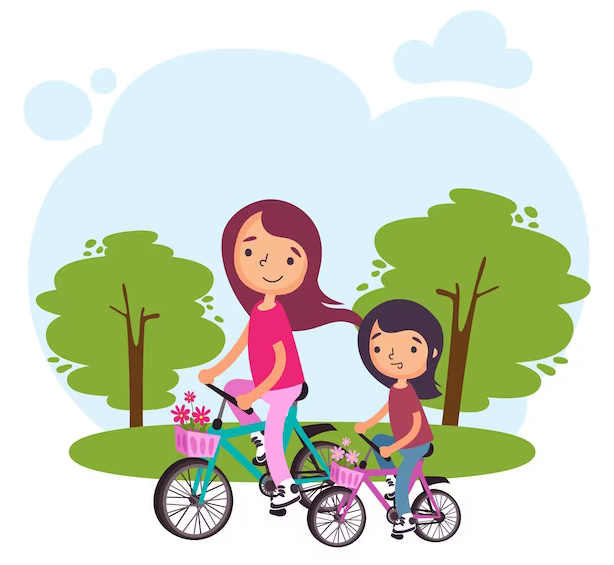
\includegraphics[width=.6\textwidth]{./media/image241.png}
\end{figure}

A FRASE QUE REPRESENTA A IMAGEM É

\begin{escolha}

\item AS MENINAS CAÍRAM DE BICICLETA.

\item AS MENINAS ANDAM DE BICICLETA.

\item AS MENINAS COMPRAM A BICICLETA.

\item AS MENINAS VENDEM A BICICLETA.

\end{escolha}

\num{9} VEJA O PRESENTE QUE MATHEUS GANHOU DE SEU AMIGO.

\begin{figure}[H]
\centering
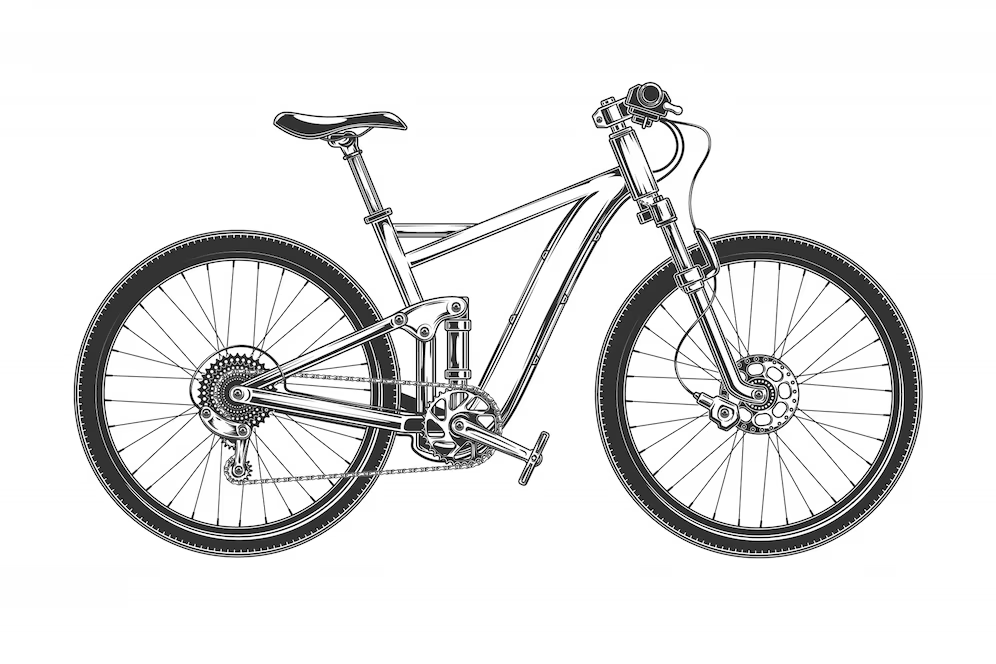
\includegraphics[width=.7\textwidth]{./media/image242.png}
\end{figure}

\pagebreak
A SEPARAÇÃO SILÁBICA DO NOME DA FIGURA É

\begin{escolha}

\item BI-CICL-ETA

\item BICI-CLE-TA

\item BICI-CL-E-TA

\item BI-CI-CLE-TA

\end{escolha}

\num{10} BETO, ANITA, CAIO E JOCA ESTÃO BRINCADO DE BAFO.
VEJA A QUANTIDADE DE CARTAS DE CADA UM.

\begin{table}[H]
\centering
\begin{tabular}{|c|c|}
\hline
\textbf{CRIANÇAS} & \textbf{QUANTIDADE DE CARTAS} \\ \hline
BETO              & QUATRO                        \\ \hline
ANITA             & OITO                          \\ \hline
CAIO              & NOVE                          \\ \hline
JOCA              & SETE                          \\ \hline
\end{tabular}
\end{table}

QUAL CRIANÇA TEM NOVE CARTAS?

\begin{escolha}

\item JOCA.

\item CAIO.

\item BETO.

\item ANITA.

\end{escolha}

\num{11} OBSERVE A IMAGEM A SEGUIR.

\begin{figure}[H]
\centering
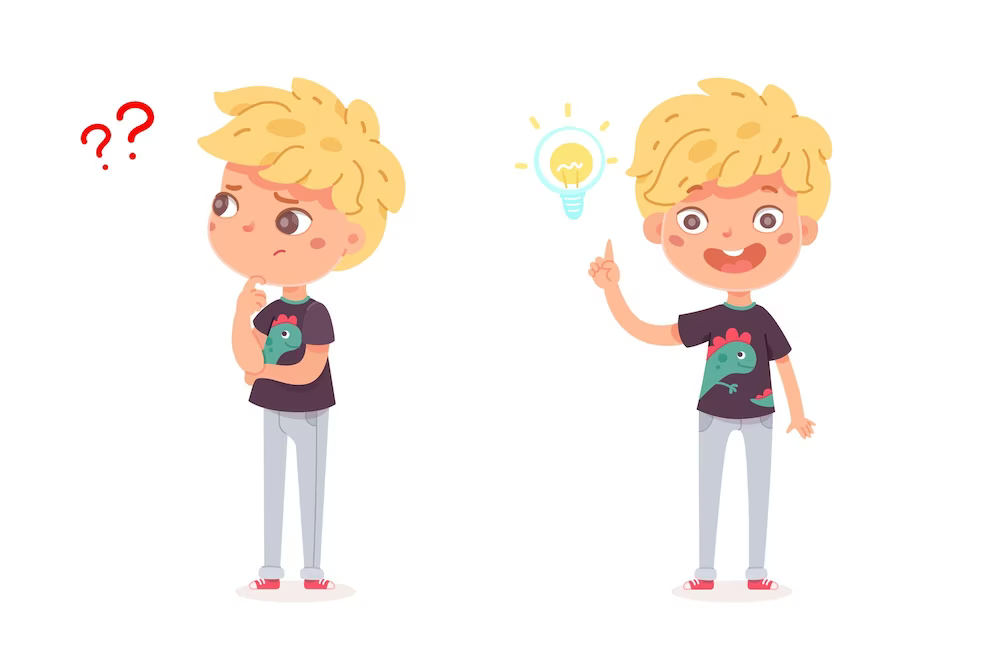
\includegraphics[width=.8\textwidth]{./media/image243.png}
\end{figure}

A FIGURA RETRATA QUE O GAROTO

\begin{escolha}

\item ESTÁ DORMINDO.

\item TEVE UMA IDEIA.

\item ESTÁ TRISTE.

\item ESTÁ BRINCANDO.

\end{escolha}

\num{12} OBSERVE O CARTAZ A SEGUIR.

\begin{figure}[H]
\centering
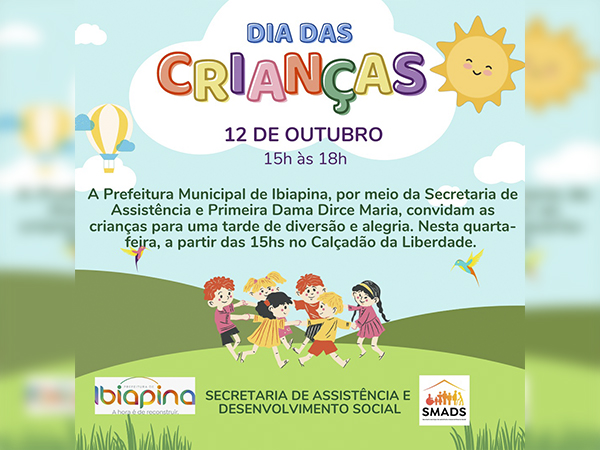
\includegraphics[width=.8\textwidth]{./media/image244.jpg}
\end{figure}

ESSE TEXTO SERVE PARA

\begin{escolha}

\item INFORMAR SOBRE A FESTA DAS CRIANÇAS.

\item CONVIDAR PARA A FESTAS DAS CRIANÇAS.

\item ENSINAR UMA BRICADEIRA PARA AS CRIANÇAS.

\item ORGANIZAR AS BRINCADEIRAS QUE SERÃO REALIZADAS.

\end{escolha}

\num{13} LEIA O TEXTO A SEGUIR.

\begin{myquote}
\textbf{A LEBRE E A TARTARUGA}

ERA UMA VEZ... UMA LEBRE E UMA TARTARUGA.
A LEBRE VIVIA CAÇOANDO DA LERDEZA DA TARTARUGA.
CERTA VEZ, A TARTARUGA JÁ MUITO CANSADA POR SER ALVO DE GOZAÇÕES, DESAFIOU A LEBRE PARA UMA CORRIDA.
A LEBRE MUITO SEGURA DE SI, ACEITOU PRONTAMENTE.
NÃO PERDENDO TEMPO, A TARTARUGA POIS-SE A CAMINHAR, COM SEUS PASSINHOS LENTOS, PORÉM, FIRMES.
LOGO A LEBRE ULTRAPASSOU A ADVERSÁRIA, E VENDO QUE GANHARIA FÁCIL, PAROU E RESOLVEU COCHILAR.
QUANDO ACORDOU, NÃO VIU A TARTARUGA E COMEÇOU A CORRER.
JÁ NA RETA FINAL, VIU FINALMENTE A SUA ADVERSÁRIA CRUZANDO A LINHA DE CHEGADA, TODA SORRIDENTE.

\fonte{https://pt.wikipedia.org/wiki/A\_Lebre\_e\_a\_Tartaruga. Acesso 12 Mar 2023.}
\end{myquote}

A MORAL DESSA HISTÓRIA, DE ACORDO COM O RESULTADO DA CORRIDA, É

\begin{escolha}

\item NÃO CONTE VITÓRIA ANTES DO TEMPO.

\item OS MAIS RÁPIDOS SEMPRE VENCEM.

\item OS FORTES CONSEGUEM O QUE QUEREM.

\item NO FIM, O MAIOR SEMPRE VENCE.

\end{escolha}

\num{14} LEIA O TEXTO A SEGUIR.

\begin{myquote}
\textbf{A MENINA DAS ESTRELAS}

VANESSA ESTAVA MUITO ANIMADA NO DIA DO SEU ANIVERSÁRIO. PASSOU A TARDE DESEMBRULHANDO PRESENTES. UAU!! ERA UM LIVRO. O PRIMEIRO LIVRO DE VANESSA. ELA FICOU MUITO CURIOSA COMO QUE PODERIA ESTAR ESCRITO ALI.
ANTES DE DORMIR, A MAMÃE LEU O LIVRO PARA VANESSA. ERA SOBRE UMA GAROTINHA QUE MORAVA NO ESPAÇO E TINHA SEU PRÓPRIO FOGUETE. VANESSA FICOU ENCANTADA. A MÃE TINHA O COSTUME DE OLHAR O CÉU PELA JANELA DA CASA. ELA COMEÇOU A JUNTAR COISAS QUE NA CABEÇA DELA TINHAM A VER COM O CÉU: PAPEL ALUMÍNIO, PEDRINHAS, DESENHOS FEITOS COM TINTA GUACHE.

\fonte{http://educacao.diadema.sp.gov.br/educacao/ Acesso 12 Mar 2023.}
\end{myquote}

\pagebreak
A MÃE LEU O LIVRO PORQUE VANESSA NÃO

\begin{escolha}

\item SABE LER.

\item GOSTA DE LER.

\item ENXERGA BEM.

\item ESTAVA COM SONO.

\end{escolha}

\num{15} OBSERVE A IMAGEM A SEGUIR.

\begin{figure}[H]
\centering

\includegraphics[width=.8\textwidth]{./media/image245.png}
\end{figure}

DE ACORDO COM A IMAGEM, O BICHO-PREGUIÇA ESTÁ

\begin{escolha}

\item TRISTE.

\item GRITANDO.

\item BRINCANDO.

\item DORMINDO.

\end{escolha}